%!TEX root = /Users/jeremy/Developpement/these/main.tex
\chapter{État de l'art}

\label{chap:etat_art}

Ce chapitre présente l'état de l'art des travaux existants sur la génération de représentations accessibles de données géographiques pour les personnes aveugles et malvoyantes. Nous commençons par définir la déficience visuelle et les mécanismes cognitifs mobilisés par les personnes concernées pour se repérer dans l'espace urbain. Nous abordons ensuite les pratiques des professionnels qui accompagnent les personnes concernées dans leur déplacement. Nous nous intéressons ensuite aux données géographiques et à leur accessibilité, en définissant ce qu'est une donnée d'accessibilité et en présentant les bases de données existantes. Enfin, nous abordons les travaux existants qui s'intéressent à la génération de représentations tactiles et textuelles de données géographiques, en particulier celles qui concernent les carrefours.

\section{Se repérer dans l'espace urbain pour une personne déficiente visuelle}

%
% Qu'est-ce que la déficience visuelle ? Comment différencier malvoyants et non-voyants ? Qu'est-ce qu'un résidu visuel ?
%

La déficience visuelle correspond à la perte de tout ou partie de la vue. On quantifie la capacité à discriminer les objets à l'aide de l'indicateur d'acuité visuelle. Ce dernier est notamment utilisé par l'\gls{oms} pour définir la déficience visuelle, et au-delà la malvoyance et la cécité. Ainsi, on parle de malvoyance lorsque l'œil le plus performant après correction a un score inférieur ou égal à 3/10\up{ème}, et de cécité lorsqu'il a un score inférieur à 1/20\up{ème}. L'étude Homère \citep{homere_2023}, qui s'intéresse à l'impact de la déficience visuelle sur la qualité de vie des personnes concernées, montre que les personnes aveugles et malvoyantes sévères (<<~acuité visuelle inférieure à 1/10\up{ème} et supérieure ou égale à 1/20\up{ème} au meilleur œil après correction~>>) sont significativement plus impactées dans leurs déplacements en autonomie que les malvoyants moyens (<<~acuité inférieure à 3/10\up{ème} et supérieure ou égale à 1/10\up{ème} au meilleur œil après correction~>>) et avec une acuité visuelle supérieure. Par ailleurs, la présence de handicaps associés (troubles moteurs, cognitifs, auditifs) peut également contribuer à rendre le déplacement plus difficile, et nécessite une prise en compte de besoins spécifiques.

\newpar{}

Dans cette thèse, nous nous intéressons aux déplacements des personnes aveugles et malvoyantes sévères, ayant éventuellement des handicaps associés. Nous utiliserons le terme \gls{pcdv} pour les désigner.

\subsection{Les mécanismes cognitifs mobilisés par les \glsentryname{pcdv}s}

%
% Stratégies de déplacement (technique de la canne blanche, chien guide, écholocation)
%

Plusieurs stratégies sont mises en place par les personnes concernées lors de leur déplacement pour compenser l'absence de vision à l'aide des autres sens. La principale stratégie concerne la canne blanche, qui joue un rôle double. Elle permet en premier lieu de détecter les obstacles et objets présents sur son chemin. Mais elle joue également un rôle social en signalant aux autres usagers que la personne qui la porte est aveugle ou malvoyante \citep{ratelle_manuel_2019}. Par ailleurs, il existe des cannes blanches électroniques, équipées de capteurs pouvant détecter des obstacles à distance (voir partie \ref{ea_dispositifs_in_situ}). Ces dernières sont cependant moins utilisées que leur variante traditionnelle \citep{homere_2023}. 

\newpar{}

Mais la canne blanche n'est pas suffisante pour se repérer dans l'espace. Son champ d'action se limite à une surface réduite face à l'utilisateur. Elle est complétée par l'ouïe qui va permettre à la personne d'appréhender l'espace en écoutant les sons de l'environnement urbain. Détecter un moteur à l'arrêt peut par exemple permettre de repérer un passage piéton en aval d'une voiture. Les dispositifs sonores en ville qui équipent certains feux vont permettre à la fois de repérer une traversée, mais également de la réaliser en sécurité (voir partie \ref{ea_dispositifs_in_situ}). L'ouïe joue également un rôle fort dans l'écholocation\footnote{On parle aussi d'écholocalisation, mais l'anglicisme écholocation est globalement plus utilisé par les personnes concernées et les professsionnels.}, c’est-à-dire la capacité à utiliser les échos pour percevoir les objets \citep{Brazier2008}. Les \glspl{pcdv} peuvent utiliser l'écholocation passive, c'est-à-dire en écoutant les sons de l'environnement, mais aussi active en émettant un son (en général un clic avec la bouche) pour en percevoir l'écho \citep{thaler2016}.

% Au-delà de l'écholocation, parler de proprioception

% Les outils de l'autonomie : carte mentale PCF, solutions techniques type GPS

\newpar{}

Dans le processus d'appropriation de l'espace, la cognition spatiale est un élément central qui peut être structuré autour d'une carte mentale. Une carte mentale correspond à un modèle conceptuel d'un espace et des objets qui le composent \citep{Jacobson1998}. Elle encode notamment leurs propriétés métriques et leurs relations topologiques \citep{Denis1992}. Ainsi, pour se déplacer en autonomie dans un environnement urbain, il faut avoir conscience de la position relative des espaces connus pour pouvoir s'orienter. Cette carte mentale est fortement alimentée par la vue pour une personne voyante, les repères visuels dans l'espace public étant beaucoup plus nombreux \citep{thinus1997}. Ne pouvant pas compter sur la vue, les \glspl{pcdv} utilisent principalement l'ouïe et le toucher au cours de leurs trajets pour percevoir leur environnement. Cependant, la construction de la carte mentale d'un lieu peut également s'opérer ex situ, par exemple à l'aide de descriptions verbales détaillées ou de cartes en relief (voir parties \ref{ea_description_autosuffisante} et \ref{ea_cartetactile}).

\newpar{}

Un aspect important de cette carte mentale concerne les repères. Ceux-ci vont permettre, à l'aide des notions d'indices et de preuves \citep{Giudice2010}, de confirmer sa position et sa direction. Les repères peuvent faire appel au sens du toucher (un objet que l'on va sentir à la canne), de l'ouïe (une fontaine en fonctionnement), ou de l'odorat (une boulangerie ouverte). On peut également définir un repère à l'aide de trois attributs: Permanent, Caractéristique et Fiable (PCF) \citep{Denis2023}. Ainsi, un repère qui respecte ces trois critères sera tout le temps mobilisable, au contraire d'une fontaine ou d'un commerce qui peuvent être intermittents. 

% La carte mentale peut être alimentée par les déplacements habituels des personnes qui repèrent l'environnement. Mais elle peut également l'être à l'aide de différents dispositifs. Une carte tactile peut aider à comprendre un espace non familier. Mais les personnes peuvent également utiliser un GPS piéton qui pourra décrire en cours de route l'itinéraire, l'infrastructure et les points d'intérêt croisés sur le chemin.

% Parler des causes de la déficience visuelle (DMLA, accident) ? Pourquoi parle-t-on de handicaps associés (conclusion de la sous-partie) ?

\subsection{Les pratiques des \ipas{}}

\label{pratiques_ipas}

L'\gls{afiadv} est issue de la fusion de l'\gls{aildv} et de l'\gls{avjadv} opérée en 2021. Ces dernières formaient respectivement les \glspl{il} et les \glspl{iavj}. L'\gls{afiadv} forme aujourd'hui des \glspl{ia} dont la profession regroupe les deux expertises précédentes. Il y a peu de littérature francophone sur les pratiques des \glspl{il}, dont le métier était uniquement centré sur la locomotion. Les actuels \glspl{ia} correspondent davantage au modèle nord-américain des instructeurs en orientation et mobilité. À ce titre, le manuel d'orientation et mobilité proposé par \citet{ratelle_manuel_2019} est une référence actuelle sur les pratiques de la nouvelle génération d'instructeurs en France.

\begin{figure}[ht]
    \centering
    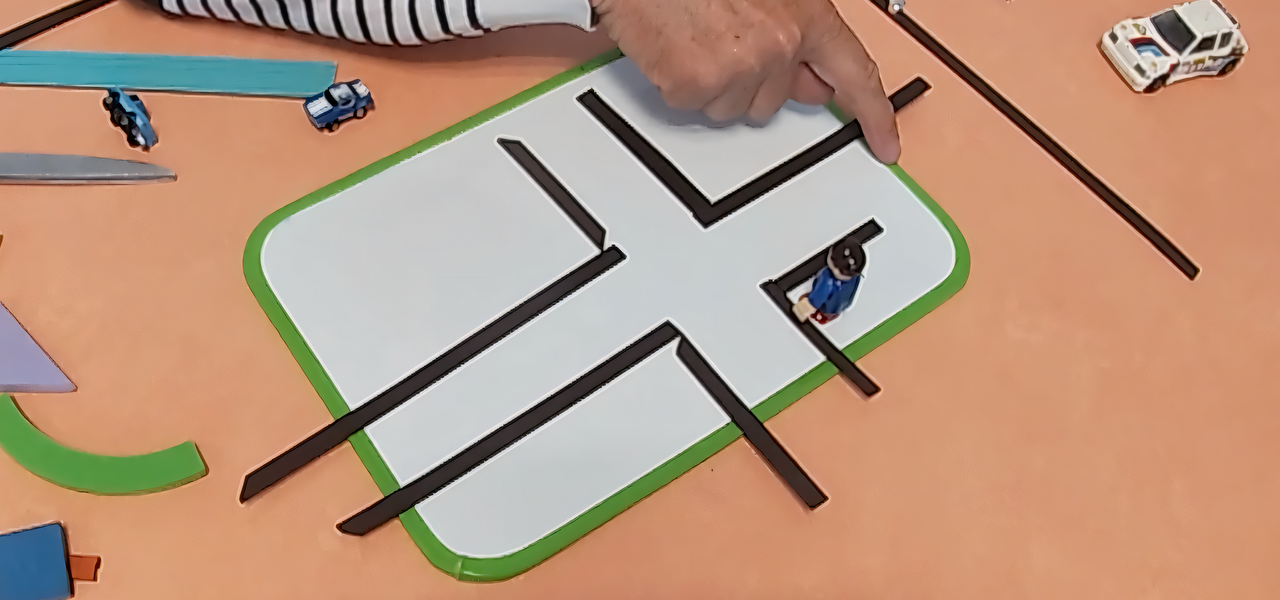
\includegraphics[width=\textwidth]{images/etat_art/carte_didier.png}
    \caption[Carte tactile produite avec des aimants]{Une carte tactile produite par un instructeur avec des aimants et des objets mobiles pour explorer la configuration d'un carrefour. Source: \gls{activmap}.}
    \label{fig:il_carte}
\end{figure}

\newpar{}

Dans ce contexte, le rôle de l'\gls{ia} est d'accompagner la personne aveugle ou malvoyante dans la compensation de la perte de la vue par l'usage des autres sens. Elle peut, pour cela, mobiliser des cartes en relief. S'il existe des outils de conception automatisée (voir partie \ref{ea_cartetactile}), la pratique de réalisation des cartes en relief est aujourd'hui majoritairement artisanale. Lors d'une séance de locomotion, un \gls{ia} réalise parfois une carte de situation en utilisant des aimants (voir figure \ref{fig:il_carte}). Ce dispositif permet notamment une interaction avec l'apprenant qui peut les déplacer selon sa compréhension du lieu. Pour représenter une zone plus complexe et faire une carte plus exploratoire, les \glspl{ia} réalisent des cartes imprimées sur du papier thermogonflé. Ne disposant généralement pas de compétences spécifiques en cartographie, les \glspl{ia} réalisent ces cartes au sein de traitements de textes ou d'outils de dessins vectoriels pour décalquer une photographie aérienne, en complétant les zones couvertes par la végétation par leur connaissance du terrain. 

\section{Les données géographiques et l'accessibilité}

La dimension géographique des données est un élément central dans la conception de cartes et de dispositifs d'aide au déplacement. Dans cette partie, nous nous intéressons à la manière dont les données géographiques peuvent être modélisées pour représenter l'accessibilité, et aux bases de données existantes. 

\subsection{Que sont les données d'accessibilité ?}

% Définir les données géographiques et leur type : couche, graphe, etc.

Dans un \gls{sig}, les données sont généralement représentées sous la forme de couches dont l'empilement compose la carte, à la manière des logiciels de dessin assisté par ordinateur (voir figure \ref{fig:geodatalayers}). On distingue principalement les données raster et les données vectorielles. Les premières correspondent à une grille dont chaque cellule contient une valeur, et permettent de stocker par exemple des images ou des reliefs. Les secondes correspondent à des données structurées ou non auxquelles est accolée une abstraction géométrique de la réalité. Il s'agit principalement de données tabulaires avec une ou plusieurs colonnes de géométrie, ces dernières pouvant être des points, des lignes ou des polygones. Une couche correspond ainsi à une table telle qu'on peut la définir dans un \gls{sgbdr} \citep{AschanLeygonie2019}. Le paradigme en couches n'est pas la seule manière de représenter les données géographiques: il est par exemple possible de les représenter sous forme de graphe, comme le propose notamment \gls{osm} (voir partie \ref{sec:modelisation_osm}).

\begin{figure}[ht]
    \centering
    \resizebox{10cm}{!}{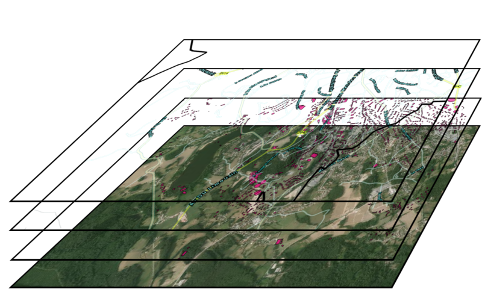
\includegraphics{images/layers.png}}
    \caption[Représentation en couche des données géographiques]{Représentation en couches des données géographiques.}
    \label{fig:geodatalayers}
\end{figure}

\newpar{}

% Parler des dispositifs d'accessibilité (BEV, etc., voir CEREMA): pas d'exhaustivité sur les dispositifs, précision plus forte dans Modélisation

Une donnée d'accessibilité est une donnée géographique qui décrit les conditions d'accès d'un lieu au regard des nécessités des personnes ayant des besoins spécifiques, comprenant les personnes en situation de handicap, mais également les personnes avec une poussette ou un bagage \citep{Ding2014}. L'espace urbain dispose d'infrastructures pour permettre à une \gls{pcdv} de se repérer et de confirmer le cheminement qu'elle suit. À ce titre, en France, le \gls{cerema} produit des documents techniques à destination des aménageurs pour les informer sur les dispositifs existants et les bonnes pratiques pour les implanter (voir figure \ref{fig:ea_exemple_cerema_bev}).

\begin{figure}[ht]
    \centering
    \resizebox{\linewidth}{!}{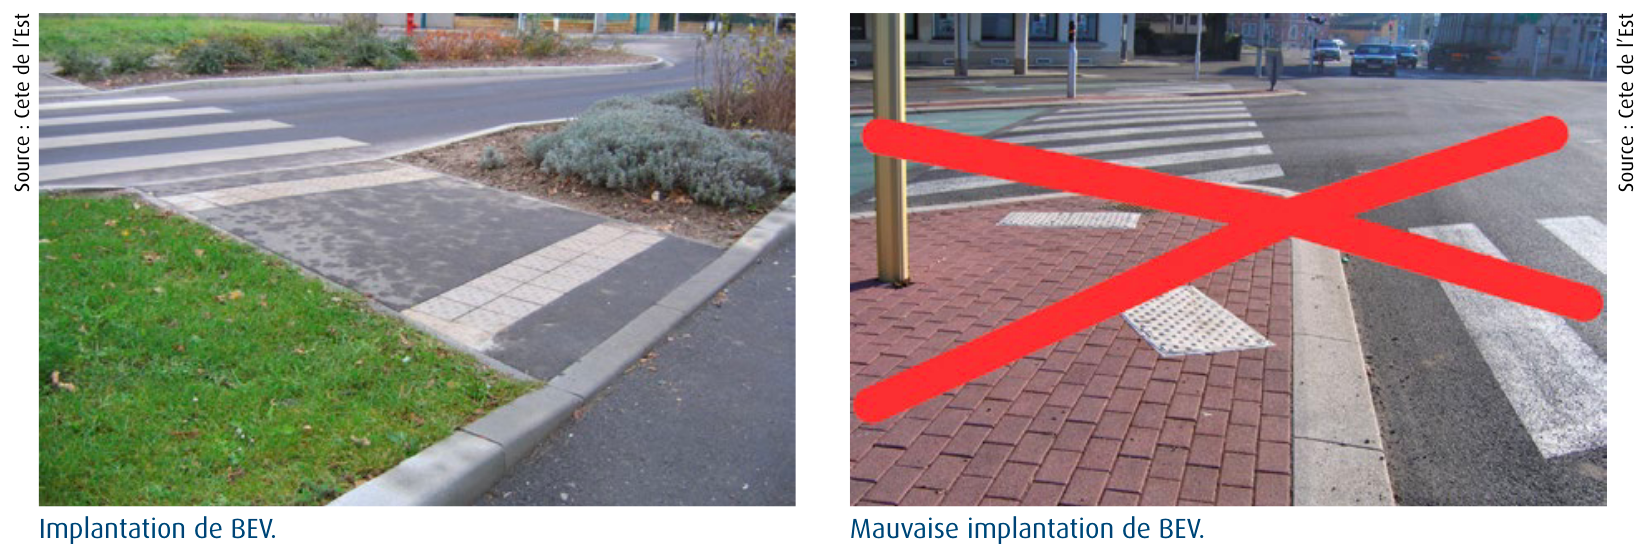
\includegraphics{images/ea_exemple_cerema_bev.png}}
    \caption[Bonnes pratiques d'implantation des pavages tactiles]{Exemple issu du \gls{cerema} sur les bonnes pratiques d'implantation de \gls{bev}. Source: \citep{CEREMA2022}.}
    \label{fig:ea_exemple_cerema_bev}
\end{figure}

% Parler des modèles de données qui permettent de contenir des informations sur l'accessibilité
% Netex, Géostandard, CityGML

\newpar{}

% Je reprécise 
% Je cite les principaux modèles (note de bas de page pour citer d'autres modèles -CityJSON-).
% Géostandard, NeTEx, GTFS, CityGML, OSM

\newpage
Les modèles de données standardisés utilisés dans les domaines de l'urbanisme et du transport peuvent intégrer une dimension liée à l'accessibilité. En France, la \gls{lom}, promulguée en 2019, impose aux collectivités de collecter et publier les données d'accessibilité de la voirie à 200 mètres autour des arrêts de transports en commun. Le formalisme utilisé, le géostandard accessibilité normalisé par le \gls{cnig}, est un dérivé du \gls{netex} pensé pour la description fine des cheminements piétons, ces derniers pouvant être représentés sous la forme de linéaire indépendants du réseau routier et embarquant une sémantique décrivant des attributs liés à leur accessibilité. Le \gls{netex} est un format européen de description des réseaux de transports qui couvre un périmètre fonctionnel plus large que le géostandard du \gls{cnig}. Le \gls{netex} permet déjà de représenter les cheminements piétons, mais avec une précision sémantique moindre. Il vise à supplanter en Europe la norme \gls{gtfs}, prévue pour le même usage, mais moins précise sur les questions d'accessibilité. D'autres formalismes plus généraux peuvent être mobilisés. CityGML \citep{Groeger2012}, pensé pour proposer une représentation 3D de l'espace urbain, est prévu pour être étendu à des usages spécifiques \citep{Biljecki2018}. Cette possibilité est par exemple exploitée par \citet{Wheeler2020} pour y intégrer les cheminements piétons et leurs conditions d'accessibilité.

\subsection{Les bases de données existantes}

% Parler des données modélisées mais non-disponibles (cycle des feux)
% Parler des données temporelles (travaux)

L'acquisition des données géographiques est un processus généralement mené par des professionnels. Cela est également vrai pour les données d'accessibilité pour lesquelles la précision demandée nécessite une opération manuelle particulièrement longue et des relevés sur le terrain \citep{Beale2006}. En France, la disponibilité de ces données d'accessibilité est essentiellement éparpillée au sein des portails de données ouvertes de chaque collectivité. On peut par exemple évoquer le portail Paris Data\footnote{https://opendata.paris.fr} qui donne accès à une donnée sur les trottoirs précise, ainsi qu'à des données temporelles utiles dans un contexte de mobilité telles que la présence de travaux sur la voie. Cependant, les modèles utilisés sont aujourd'hui propres à chaque collectivité, et leur disponibilité et leur précision varient d'un territoire à l'autre \citep{Ding2014}.

% Parler du travail d'Eunice

\newpage

L'émergence de l'\gls{igv} a apporté une nouvelle perspective à la collecte de données, permettant d'augmenter leur disponibilité sur des zones et des thèmes auparavant peu couverts \citep{Goodchild2007}, dont l'accessibilité. \gls{osm} est une base de données géographique généraliste, libre et collaborative couvrant une échelle mondiale. Son modèle repose sur un système de clés-valeurs\footnote{Sur \gls{osm}, une clé est nommée tag.} souple, dont les associations permettent de décrire une très grande diversité d'objets. L'utilisation des clés et leur valeur associée pour un objet est discutée et documentée \citep{Ballatore2015} sur le wiki du projet\footnote{https://wiki.openstreetmap.org}. Sur \gls{osm}, \citet{Mobasheri2017} montre que les données d'accessibilité sont également éparses, leur complétude pouvant varier d'une ville à l'autre. Par ailleurs, leur modélisation et leur précision sont également hétérogènes \citep{Biagi2020} en ce qui concerne les trottoirs.

% Justification utilisation OSM : plein de paradigmes de modélisation de cartographie fine (CityGML, Netex, etc.). Le plus fexible pour nos besoins = OSM.

\section{Les représentations accessibles de données géographiques}

% Dans cette partie, chaque sous section se termine avec un focus sur l'existant au sujet des carrefours.
% Introduire les données géographiques et les bases de données les plus communes (OpenStreetMap)

Les données géographiques peuvent être utilisées pour concevoir des cartes, mais également au sein de dispositifs sensoriels permettant à une \gls{pcdv} de les explorer. Pour cela, il est nécessaire d'en proposer une représentation accessible par d'autres sens que la vue. Cette partie s'intéresse à présenter les dispositifs décrits au sein de la littérature, ainsi que ceux effectivement mobilisés dans leur quotidien par les personnes concernées.

\subsection{Les descriptions autosuffisantes}

\label{ea_description_autosuffisante}

% Voir aussi https://journals.sagepub.com/doi/10.1177/0145482X0409800802

% Définition : une description autosuffisante c'est un texte mobilisable tel quel. Il n'y a pas d'interactions entre l'utilisateur et le texte.

% Une description verbale/textuelle aide à la construction d'une carte mentale

Une carte mentale construite à partir d'une description verbale partage ses propriétés avec une carte mentale dérivée d'une expérience visuelle, dont les relations spatiales entre les entités \citep{Denis1992}. Par ailleurs, elle permet d'inférer des relations spatiales non explicitement indiquées dans la description, et ainsi d'adopter un point de vue exocentré \citep{Avraamides2004} (voir partie \ref{sec:description_textuelle}). Une description verbale peut ainsi être mobilisée par les \glspl{pcdv} afin de construire une représentation mentale d'un espace.

\newpar{}

% Concevoir une description pour une PCDV

La littérature sur la conception de description à destination de \gls{pcdv} se concentre principalement sur la description d'itinéraires. Du point de vue des sciences cognitives, de nombreux travaux se sont intéressés aux principes et pratiques pour communiquer efficacement la connaissance d’un itinéraire, en analysant les éléments qui le constituent et influent sur sa qualité \citep{Allen2000,Lovelace1999}. Les recherches qui se focalisent sur la question de la déficience visuelle abordent la description d'itinéraires en fonction des environnements intérieurs ou extérieurs.

\newpar{}

Un modèle pour la création de description d'itinéraires en intérieur est proposé par \citet{Troeger2020}. Il repose sur des descriptions validées par des utilisateurs concernés et comprend plusieurs séquences de directions augmentées de repères. Une approche similaire est abordée par \citet{Kulyukin2008} pour le guidage au sein d'un commerce, dont les descriptions sont générées automatiquement en utilisant des textes à trous complétés par les attributs du graphe topologique représentant le commerce (voir figure \ref{fig:ea_kulyukin_graph}).

\begin{figure}[ht]
    \centering
    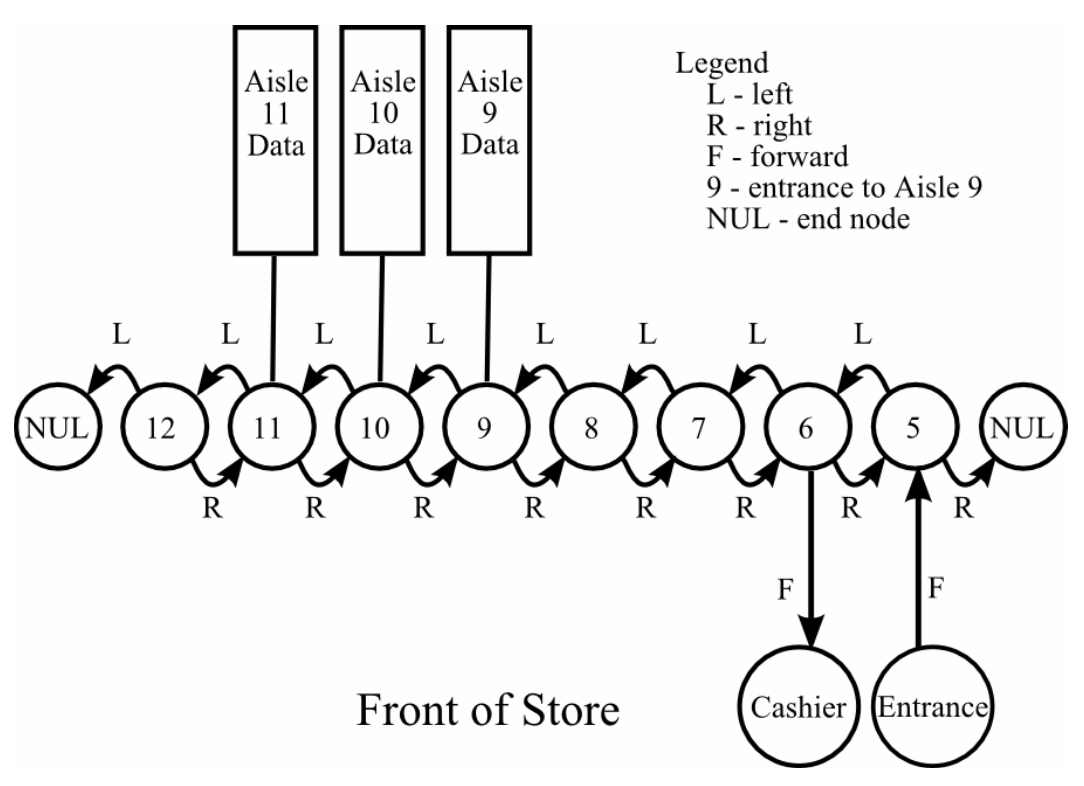
\includegraphics[width=0.5\textwidth]{images/etat_art/kulyukin_graph.png}
    \caption[Graphe topologique de l'intérieur d'un commerce]{Le graphe topologique de l'intérieur d'un commerce proposé par \citet{Kulyukin2008} est utilisé pour générer une description de celui-ci. Source: \citep{Kulyukin2008}.}
    \label{fig:ea_kulyukin_graph}
\end{figure}

\newpage{}

Pour le guidage extérieur, \citet{gaunet_verbal_2006} propose une grammaire de description d'itinéraire sous la forme de fonctions de guidage dont le déclenchement est associé à une position et un type de situation précis. Une forme verbale est associée à ces fonctions, permettant de décrire un cheminement au sein de la ville, et peut notamment comprendre une indication d’orientation angulaire ou relative à une voie de circulation (voir figure \ref{fig:ea_ex_desc_gaunet}). \citet{Balata2016} proposent une approche similaire et génèrent automatiquement les descriptions à l'aide d'un graphe piéton enrichi par des repères. Chaque instruction est basée sur un patron et déclenchée selon le type de segment parcouru.

\begin{figure}[ht]
    \centering
    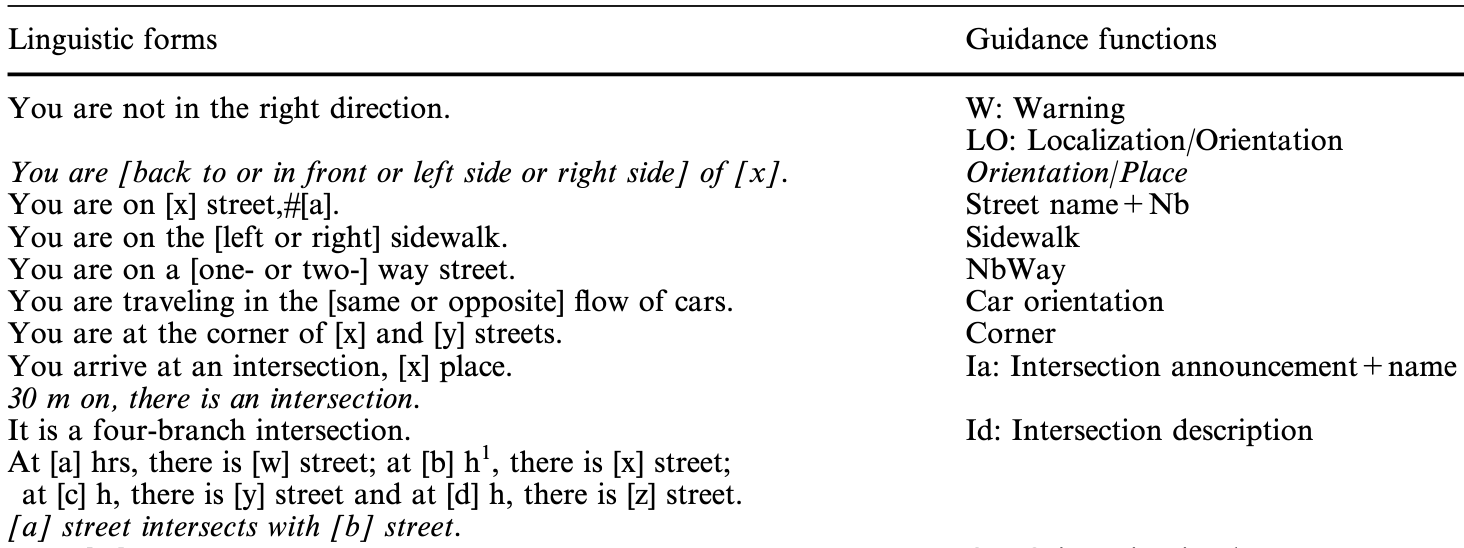
\includegraphics[width=\textwidth]{images/etat_art/exemple_itineraire_gaunet.png}
    \caption[Exemple de description issu de la littérature]{Exemple de fonctions de guidage et de formes verbales associées proposées par \citet{gaunet_verbal_2006}. Parmi celles-ci figure une description de carrefour présentant le nombre de branches et leur orientation. Source: \citep{gaunet_verbal_2006}.}
    \label{fig:ea_ex_desc_gaunet}
\end{figure}

% Quels sont les dispositifs proposant des descriptions pour le guidage (plutôt dans la partie in situ ?)

% Ce qui existe pour les carrefours

\newpar{}

Il existe peu de littérature visant spécifiquement la manière de décrire un carrefour. Cependant, la grammaire de description proposée par \citet{gaunet_verbal_2006} intègre une description basique des carrefours, indiquant leur nombre de branches ainsi que l'orientation de chacune d'elles (voir figure \ref{fig:ea_ex_desc_gaunet}).

\newpage{}

La génération automatique de description de carrefours est adressée par \citet{Guth2019}. En se basant sur la littérature en instruction et mobilité, les auteurs proposent de générer une description succincte d'un carrefour pensée pour un usage in situ. Pour cela, ils construisent deux tables de données permettant de définir respectivement pour le carrefour et chaque traversée leurs principaux attributs et l'infrastructure qui les composent. La description générée correspond à l'assemblage des différents champs de ces tables, et est découpée en une description générale du carrefour puis une description par passage piéton. Les auteurs ont choisi de remplir manuellement les tables de données, les bases disponibles sur leurs zones d'études n'étant pas satisfaisantes. Ils notent également une difficulté à choisir une terminologie adaptée, les termes de description de carrefours n'étant pas standardisés chez les \glspl{pcdv}, les \glspl{ia} et les aménageurs, et effectivement variés dans le panel des personnes participant à l'étude.

\subsection{Les cartes en relief}

Les cartes en relief (voir figure \ref{fig:excartestactiles}) permettent d'explorer une représentation de la donnée géographique accessible au toucher. Elles sont souvent réalisées manuellement par les \glspl{ia} et les adaptateurs-transcripteurs (voir partie \ref{pratiques_ipas}). La revue de littérature de \citet{Wabinski2022} rappelle qu'elles répondent à des règles de conception précises afin de permettre à leur lecteur de les comprendre et d'en distinguer les différents éléments.

\begin{figure}[ht]
    \centering
    \begin{subfigure}[t]{0.49\textwidth}
        \centering
        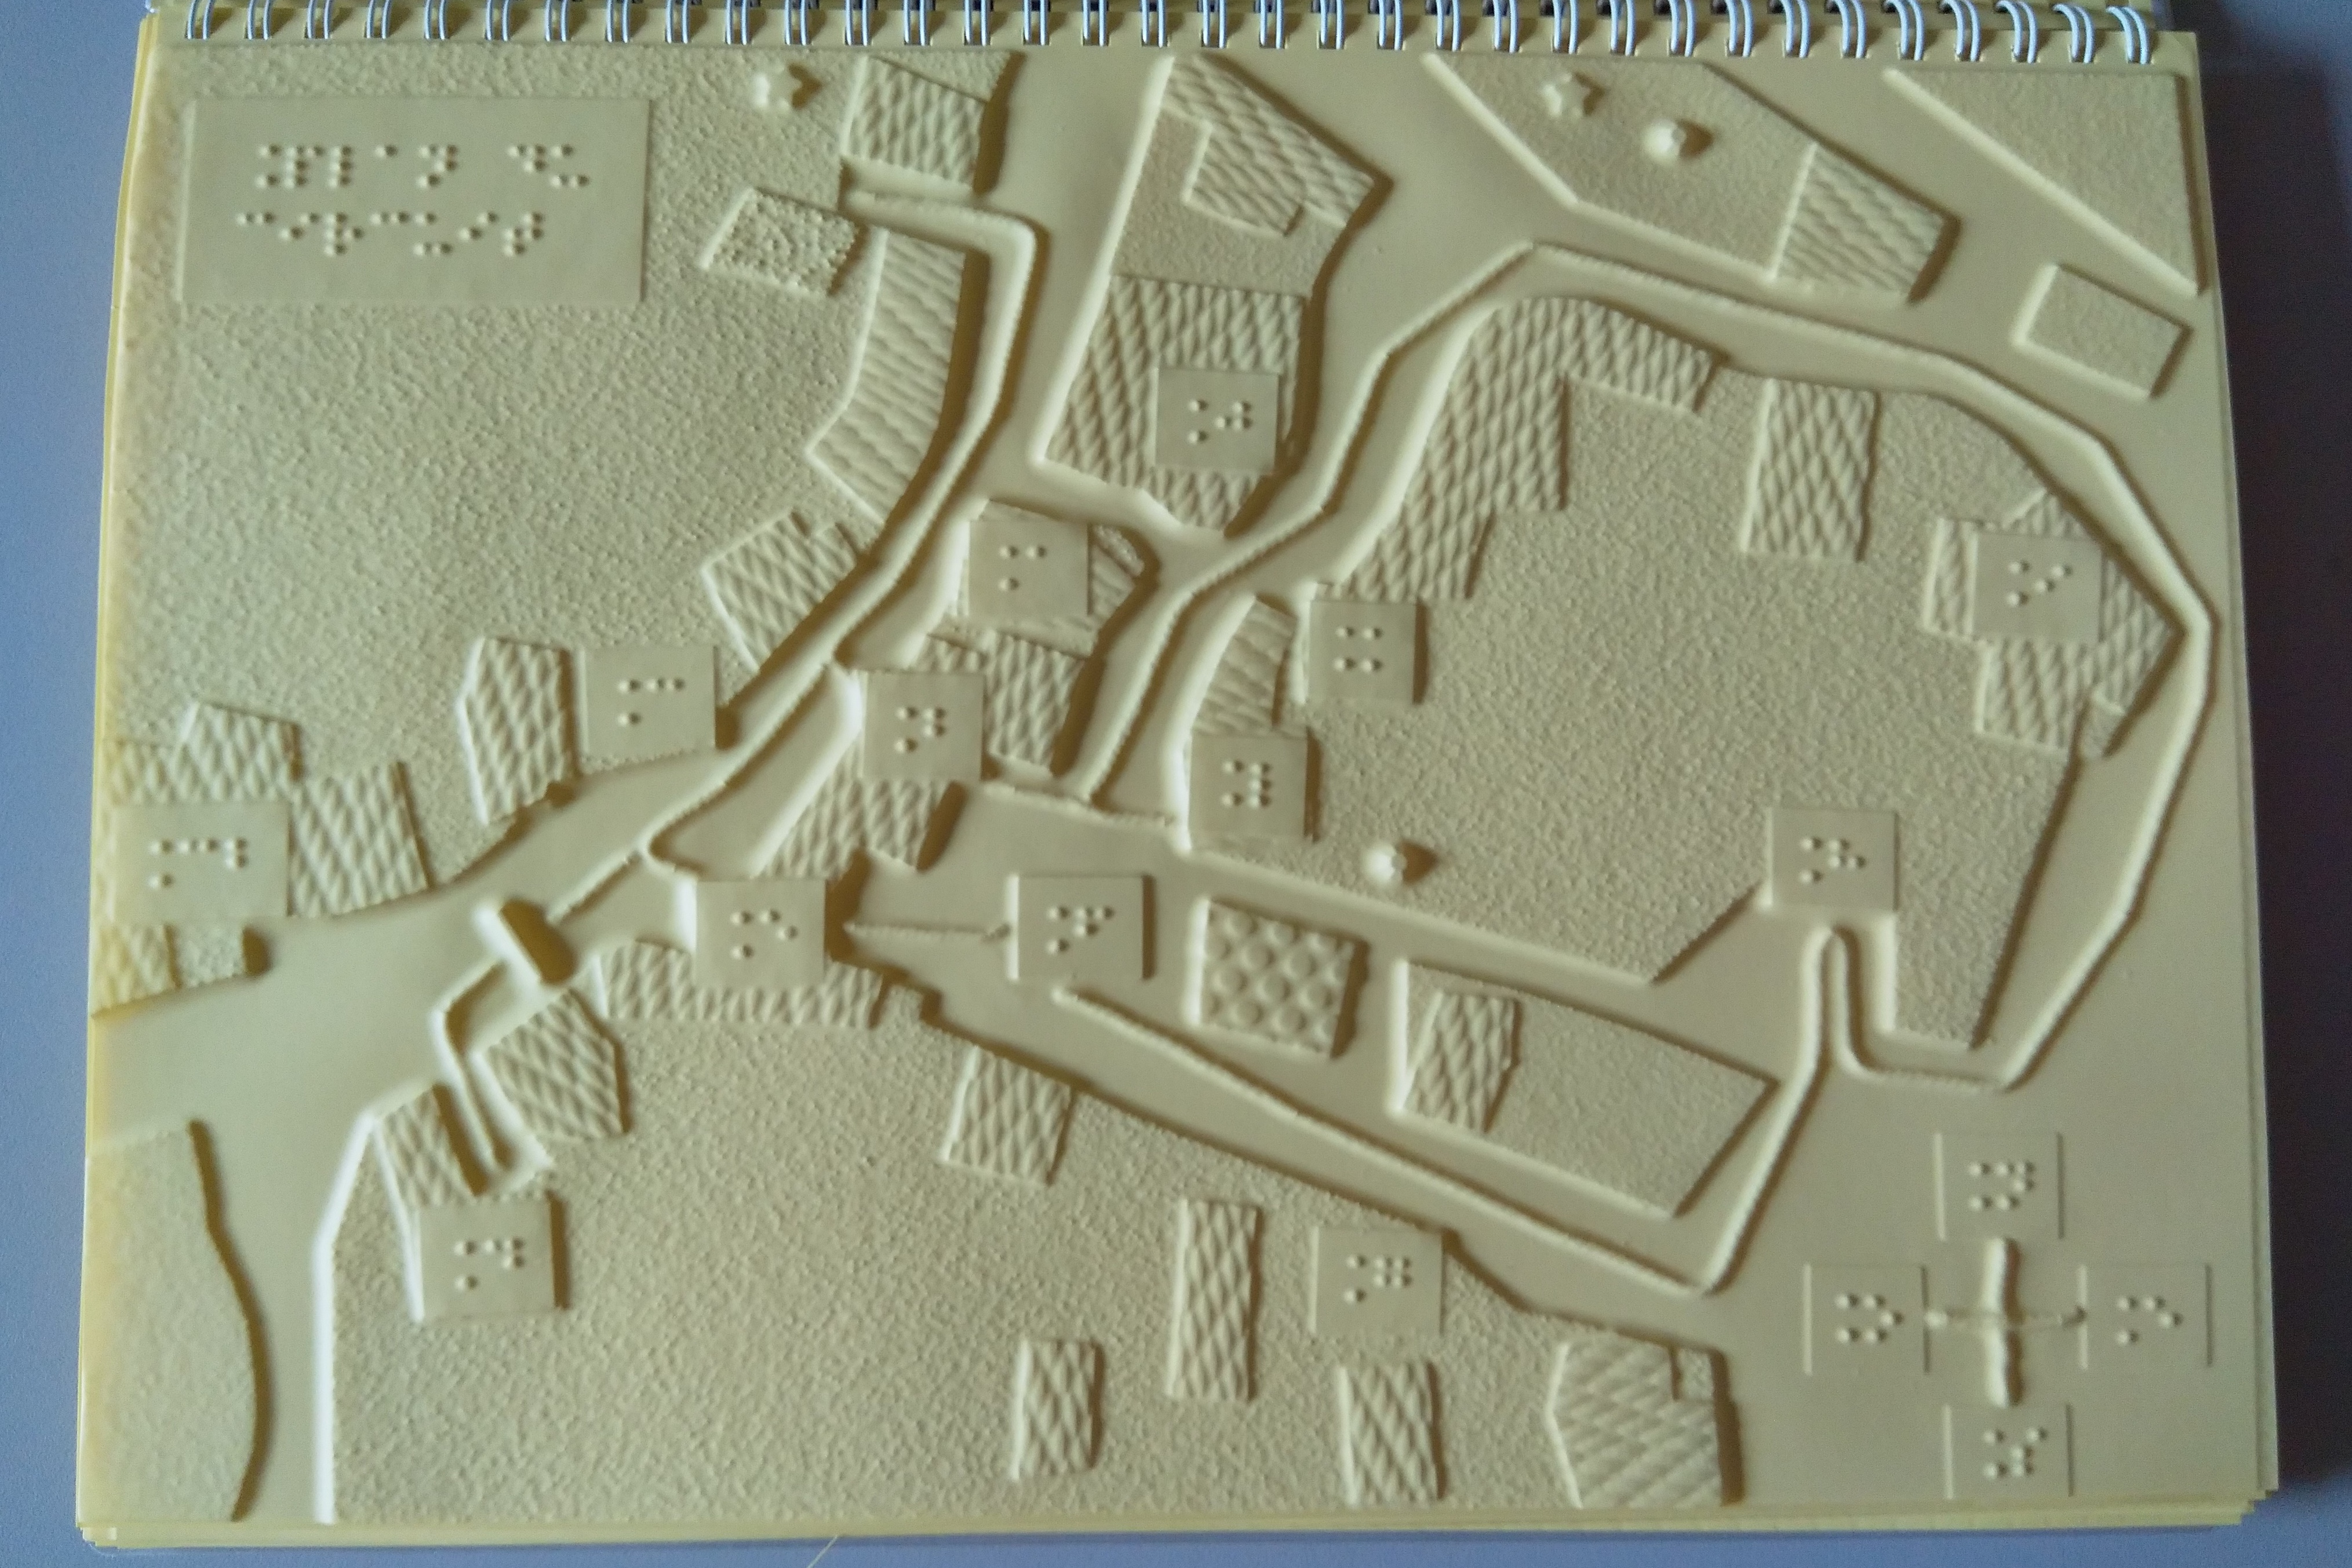
\includegraphics[width=\textwidth]{images/etat_art/carte_tf_collonges.jpg}
        \caption{Carte thermoformée de la route principale du village de Collonges-la-Rouge. Source: AcceSens\footnote{https://www.accesens.com/}.}
    \end{subfigure}
    \hfill
    \begin{subfigure}[t]{0.49\textwidth}
        \centering
        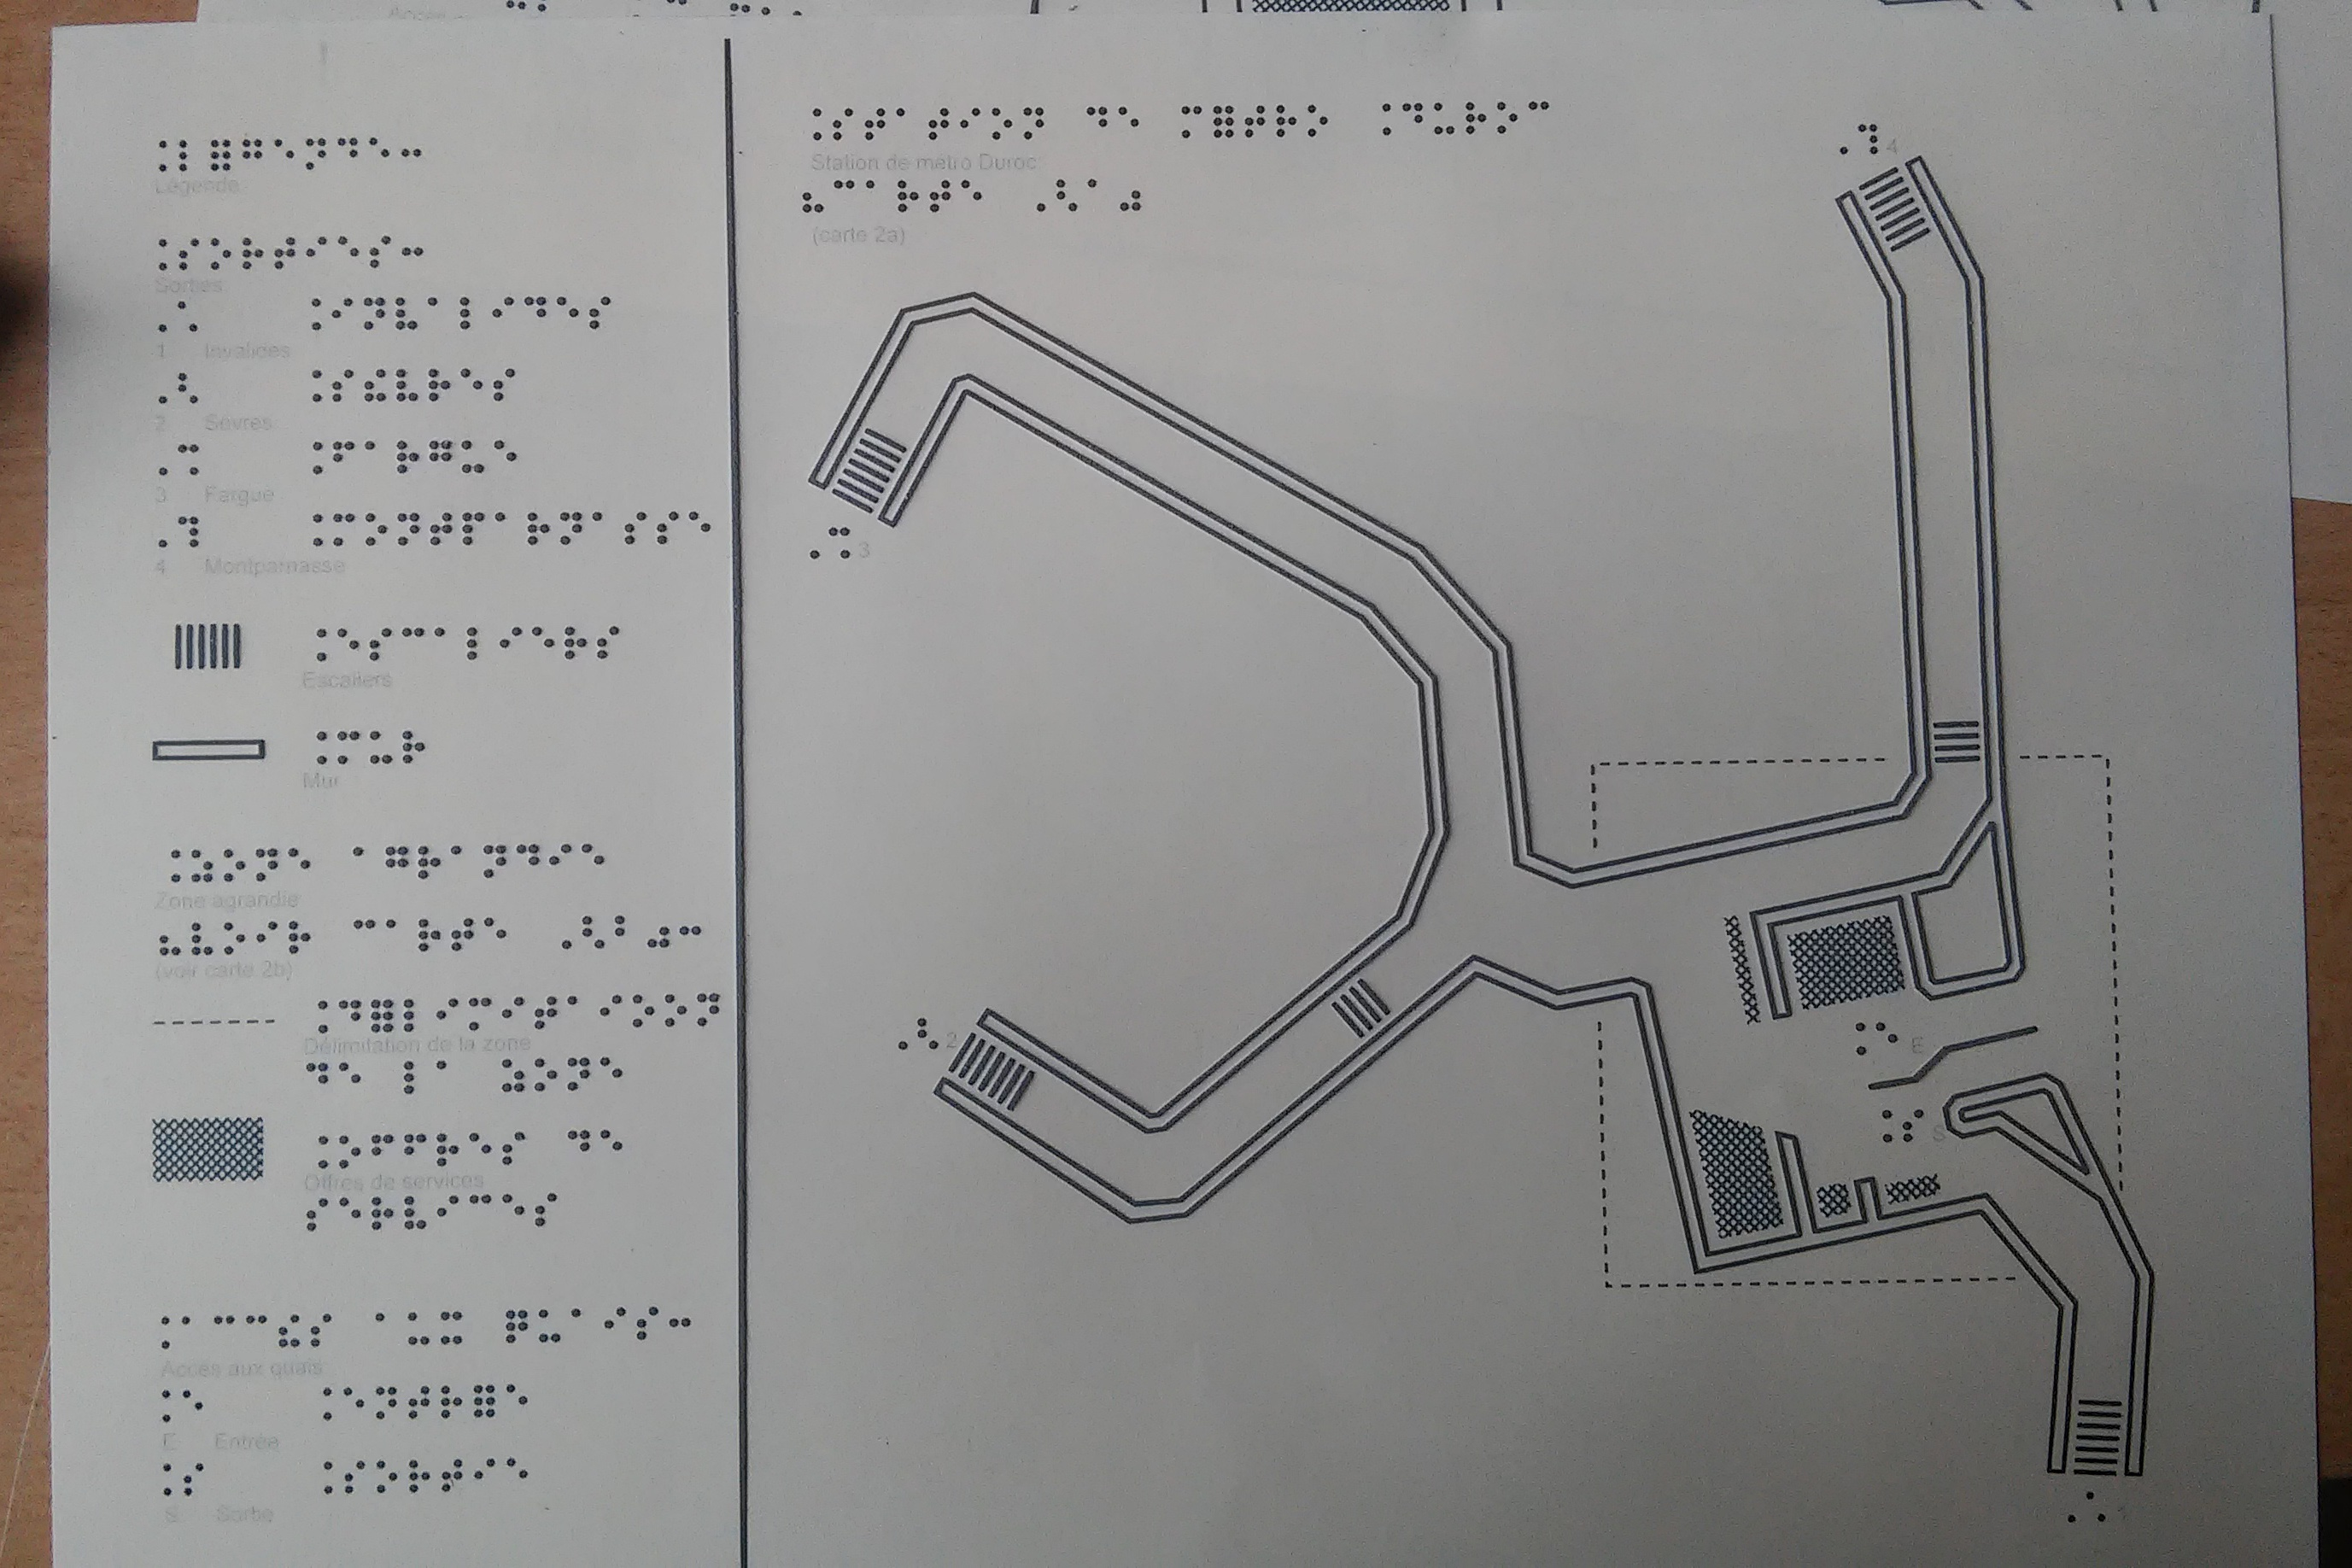
\includegraphics[width=\textwidth]{images/etat_art/carte_tg_duroc.jpg}
        \caption{Carte thermogonflée de la station de métro Duroc à Paris. Source: \gls{inja}.}
    \end{subfigure}
    \caption[Différents types de cartes en relief]{Différents types de cartes en relief. Source: collecte du projet ACCRIL\footnotemark.}
    \label{fig:excartestactiles}
\end{figure}
\footnotetext{https://compas.limos.fr/ACCRIL/}

\newpar{}

La génération automatique de cartes en relief basée sur des données géographiques présente de nombreux défis scientifiques et techniques. Une revue de littérature proposée par \citet{Wabinski2019} présente de manière exhaustive les différentes approches existantes. Si d'autres travaux ont adressé la génération de carte à petite échelle, l'état de l'art ci-dessous se concentre sur l'échelle de la rue qui est celle visée pour la conception de carte audiotactile dans le projet \gls{activmap}.

\newpar{}

La proposition de \citet{Miele2004}, TMAP, permet la réalisation à la demande de cartes tactiles de rues, représentées sous forme de géométries linéaires. Un service interactif permet à l'utilisateur de définir une emprise et de personnaliser la conception, par exemple au niveau de l'échelle et des éléments labellisés. Ces options vont servir à styliser la donnée, puis la carte est réalisée à l'aide d'une embosseuse braille\footnote{Une embosseuse braille est une imprimante qui permet de retranscrire en relief des caractères brailles. Les machines étant coûteuses et bruyantes, l'embossage tend à être remplacé par le thermogonflage.}. Cependant, les données utilisées pour générer les cartes proviennent d'une base de données limitée au territoire américain. 

\newpar{}

\citet{Minatani2010} proposent une approche équivalente sur le territoire japonais, en proposant une infrastructure technique applicable à d'autres territoires sous réserve de disponibilité de données géographiques équivalentes. La carte est cette fois réalisée par thermogonflage\footnote{Le thermogonflage consiste à imprimer un document en noir et blanc sur un papier spécial contenant des microcapsules. Ces dernières gonflent de manière uniforme sur les zones imprimées lorsque le papier est passé au four.}. Ils insistent par ailleurs sur l'intérêt des repères sensoriels, qui peuvent différer selon l'utilisateur, ce qui implique d'en permettre la personnalisation. 

\newpar{}

Les dispositifs précédents sont étendus par \citet{Watanabe2014, Cervenka2016} en utilisant la base de données \gls{osm} comme source afin de permettre la génération de carte tactile sur n'importe quel territoire.

\newpar{}

L'acuité sensorielle est beaucoup plus faible au toucher que pour la vue. Or, si les travaux évoqués jusqu'ici reposent sur une stylisation des données géographiques, les géométries de ces données n'ont cependant pas été pensées pour une représentation tactile et peuvent présenter des formes complexes difficiles à discerner. Il faut donc simplifier l'information  au maximum pour la rendre plus facilement lisible avec le doigt. \citet{Stampach2016} s'appuient sur les approches précédentes en insistant sur l’intérêt du processus de généralisation pour la bonne distinction des différents éléments qui composent la carte. Les processus de généralisation pouvant donner un résultat inadéquat, une édition manuelle de la carte reste possible.

\newpar{}

\citet{Touya2019} proposent d'aller au-delà de la généralisation pour <<~schématiser~>> la carte, c'est-à-dire en proposer une représentation abstraite plus adaptée aux zones urbaines denses. 

\newpar{}

Les bases de données vectorielles actuelles, même si elles offrent parfois une couverture mondiale, ne sont pas exhaustives sur tous les territoires pour les thèmes liés à l’accessibilité. Il est alors possible d'utiliser une imagerie aérienne suffisamment précise pour les compléter. \citet{FillieresRiveau2020} s'intéressent à cette problématique en proposant de générer des cartes en relief représentant notamment les trottoirs et les passages piétons par apprentissage profond en utilisant à la fois une photographie aérienne et un filaire de rues vectoriel. Cependant, cette méthode est limitée notamment par la présence de couverts végétaux ou d'ombres portées de bâtiments qui peuvent masquer les éléments de la voirie.

\newpar{}

Le sujet de la génération de cartes tactiles à l'échelle spécifique du carrefour est adressé au sein du projet \gls{activmap} par \citet{Jiang2023} en utilisant les données \gls{osm} et en accordant une attention particulière aux échelles et niveaux de détails requis.

\newpar{}

Les différents travaux de génération de cartes tactiles reposent sur des techniques variées. Ils ne s'intéressent pas toujours à la même échelle ni à la même emprise. et les supports de réalisation visés sont également variés (voir table \ref{tab:ea_relief}). Dans tous les cas, la carte en relief seule ne permet pas de représenter une haute densité d'informations \citep{Touya2019}, et est plus abordable lorsqu'elle est complétée d'une information sonore \citep{Brock2015}.

\begin{table}[ht]
\begin{center}
\scriptsize
\begin{tabular}{ | l | l | l | l | l | l | l | }
    Publication & Technique & Généralisé & Automatisé & Couverture & Échelle & Support \tabularnewline
    \hline
    \citep{Miele2004} & Stylisation & Non & Complet & États-Unis & Rues & Embossage \tabularnewline
    \citep{Minatani2010} & Stylisation & Non & Complet & Japon & Rues & Thermogonflage \tabularnewline
    \citep{Watanabe2014, Cervenka2016} & Stylisation & Non & Complet & Mondiale & Rues & Thermogonflage \tabularnewline
    \citep{Stampach2016} & Stylisation & Oui & Partiel & Mondiale & Rues & Thermogonflage \tabularnewline
    \citep{FillieresRiveau2020} & Apprentissage profond & Non & Complet & Mondiale & Rues & Impression 3D \tabularnewline
    \citep{Jiang2023} & Stylisation & Oui & Partiel & Mondiale & Carrefours & Thermogonflage \tabularnewline
\end{tabular}
\end{center}
\caption[Résumé de l'état de l'art sur la génération de cartes en relief]{Résumé des points abordés pour chaque entrée de l'état de l'art sur les cartes tactiles.}
\label{tab:ea_relief}
\end{table}

% Illustrer l'intérêt d'une carte audiotactile VS carte tactile classique

\label{ea_cartetactile}

\subsection{Les cartes sonores et audiotactiles}

\label{ea_cartessonores}

Un état des lieux des techniques mobilisables pour sonoriser les données géographiques est proposé par \citet{Krygier1994}, qui distingue notamment les sons réalistes, qui peuvent correspondre à une description verbale ou à un son imitant le réel, et les sons abstraits.

\newpar{}

% Les sons réalistes

Parmi les sons réalistes, on trouve notamment les paysages sonores. \citet{Porteous1985} définissent un paysage sonore comme \pquote{l'environnement sonore global d'une région}. Il représente l'ambiance sonore telle qu'elle est réellement perçue en un lieu. La proposition de \citet{Josselin2016} s'appuie sur la notion de paysage sonore pour sonoriser une carte topographique en associant un son à chaque couleur et en modulant son volume selon sa dominance dans la carte. Le son produit peut ainsi représenter un paysage sonore. Une alternative sous la forme d'une composition musicale originale est également proposée et répond plutôt à la définition d'un son abstrait tel que proposé par \citet{Krygier1994}. Ces derniers sont  modulés par des variables sonores telles que le volume ou la durée et peuvent être directement corrélés à des données. C'est l'approche choisie par \citet{Schito2018} qui proposent d'explorer les données continues telles que les Modèles Numériques de Terrain (MNT) en faisant correspondre leurs valeurs aux variables sonores.

\newpar{}

% La cartographie sonore multimodale

Les techniques évoquées ci-dessus visent à explorer des données par le son uniquement. Mais, comme le propose \citet{Krygier1994}, ce dernier peut être utilisé de concert avec un autre dispositif sensoriel pour proposer une représentation multimodale apportant une dimension supplémentaire à la visualisation, cette dernière pouvant être utilisée pour représenter une variable supplémentaire. C'est dans ce sens que \citet{Bearman2010} modélisent la précision positionnelle de bâtiments en établissant un son spécifique pour chaque valeur de cette variable. Une approche similaire \citep{Foteinou2022} s'intéresse à la durée des incendies en modulant la longueur du son joué au survol d'une entité. Ces dispositifs multimodaux utilisent une interface d'ordinateur standard pour permettre à l'utilisateur d'interagir avec la carte, rendant leur usage impossible par un utilisateur déficient visuel. Pour répondre à cette problématique, la littérature s'est intéressée à la sonorisation des cartes tactiles.

\newpar{}

% Les cartes audiotactiles

Les cartes dites audiotactiles se sont développées sur la base des dispositifs en relief interactifs. On en trouve de nombreux exemples parmi lesquels les propositions de \citet{Loetzsch1994} ou encore de \citet{Landau2001}, basées sur une interface tactile reliée à un ordinateur et permettant d'interagir avec celui-ci à l'aide d'un programme spécifique.
Talking TMAP \citep{Miele2006} est une extension de TMAP \citep{Miele2004} permettant d'interagir avec la carte pour obtenir des informations sur l'élément touché par synthèse vocale et repose sur le matériel conçu par \citet{Landau2001}. L'émergence des écrans tactiles grand public a permis la conception d'outils plus accessibles comme les \glspl{deri} \citep{Brock2015} (voir partie \ref{sec:experimentation_poc1}).

\subsection{Les dispositifs d'aide in situ}

\label{ea_dispositifs_in_situ}

% Je veux dire qu'il existe plusieurs familles d'outils : ceux qui ne nécessitent pas d'équipement extérieur à la personne (les cannes, le GPS, les applications smartphones, etc.) et les autres dispositifs comme les balises sonores et autres balises de guidage.
% Pour les balises sonores, je peux citer la norme. Pour les autres dispositifs, je peux éventuellement citer des brevets.

Pour cheminer en ville, une \gls{pcdv} peut utiliser des outils d'aides in situ pour s'orienter et éviter les obstacles. Il existe deux principales familles d'outils: les outils indépendants et ceux qui reposent sur un second équipement externe comme un capteur. L'enquête Homère, qui s'est également intéressée aux dispositifs mobilisés lors des déplacements, montre qu'une majorité des personnes concernées utilise des dispositifs d'aide in situ, en particulier les outils de navigation \citep{homere_2023}. Une revue plus exhaustive des dispositifs existants est proposée par \citet{Kuriakose2022}.

\newpar{}

% Les outils indépendants
On entend par outils indépendants les outils qui ne nécessitent pas d'équipement externe et qui peuvent donc être utilisés en tout lieu. Les principaux représentants de cette catégorie sont les outils de navigation, qui permettent à leur utilisateur de se localiser et d'obtenir un audioguidage vers une destination, comme le propose \citet{Golledge1998} avec un système de positionnement \gls{gnss} et un \gls{sig} pour guider en temps réel une \gls{pcdv}. Les questions de génération de texte pour ces usages sont abordées dans la section \ref{ea_description_autosuffisante}. Au-delà des travaux de recherche, il existe également des dispositifs spécialisés utilisables au quotidien, qu'il s'agisse d'applications mobiles (voir figure \ref{fig:dispositif_in_situ}) ou de matériels spécifiques comme les outils de navigation \glspl{gnss} \citep{Refuveille2012}. 

\begin{figure}[ht]
    \centering
    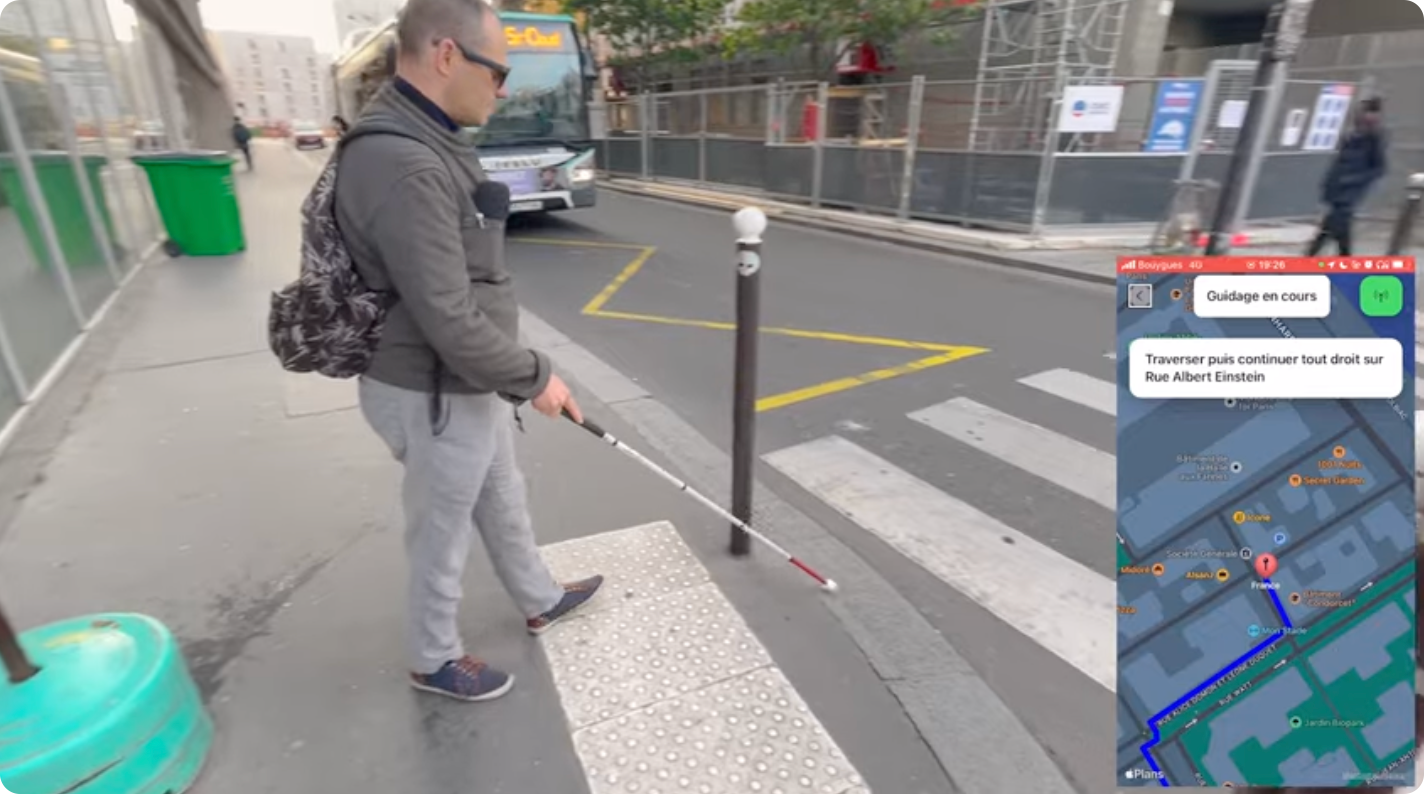
\includegraphics[width=0.8\textwidth]{images/ea_dispositifs_in_situ.png}
    \caption[Application mobile de guidage]{Sonarvision: un exemple d'application de guidage qui repose sur le \gls{gnss} et la caméra d'un smartphone. Source: \url{https://youtu.be/geGq59f11z0}.}
    \label{fig:dispositif_in_situ}
\end{figure}

\newpage{}

Les dispositifs qui se reposent sur des capteurs embarqués permettent le positionnement et la détection d'obstacles. La littérature s'est notamment intéressée aux cannes électroniques. Plusieurs dispositifs ont été étudiés pour la détection d'obstacle à l'aide de capteurs laser ou infrarouge \citep{Damaschini2005}. Certains utilisent ces capteurs pour localiser l'utilisateur sur la base d'une cartographie d'un lieu \citep{Connier2018}. Les caméras embarquées peuvent également servir d'outil de positionnement à l'aide d'algorithmes de vision par ordinateur \citep{Duh2021}.

\newpar{}

% Balises de guidage, balises sonores
D'autres outils d'aide in situ se reposent sur des dispositifs qui équipent le lieu visité. Il peut s'agir de balises de guidage qui peuvent servir d'outils d'orientation en extérieur et en intérieur \citep{Ahmetovic2016, Cheraghi2017}. \citet{Shin2022} proposent un système similaire dédié à la traversée des carrefours. Aujourd'hui, de nombreux lieux, tels que les carrefours, sont également équipés de balises sonores. Celles que l'on retrouve en France répondent à la norme NF S32-002 \citep{NFS32002_2004} et s'activent à l'aide d'une télécommande standardisée. À un passage piéton notamment, elles indiquent à quel moment le feu piéton est vert. Cependant, tous les passages piétons ne sont pas équipés de ces dispositifs, et la proximité de plusieurs balises, sur un carrefour par exemple, peut les rendre difficiles à distinguer. Par ailleurs, la fréquence d'activation des balises, 868.3 MHz, est également utilisée par d'autres dispositifs tels que les portes de garage, ce qui peut générer des interférences et rendre leur activation moins fiable \citep{Rahal2021}.

\subsection{La réalité virtuelle et les maquettes interactives}

% Définir ce qu'est la réalité virtuelle : immersion + interaction ?
% Parler des maquettes interactives (voir tangible box)
% Parler des sons immersifs, soit spatialement positionnés (salle sonore) soit virtuels (son binaural/spatial)
% Parler des outils de navigation virtuel, qui permettent une exploration à distance (livre dont vous êtes le héros)

% Références :
% - The Sound of Being There: Audiovisual Cartography with Immersive Virtual Environments, Hruby, 2019

En l'absence de vision, il existe d'autres modalités permettant d'explorer un environnement en réalité virtuelle, par le toucher et par le son. On définit ici la réalité virtuelle comme un  moyen immersif et interactif d'explorer un environnement à distance.

\newpar{}

% Le toucher, les maquettes interactives
Les cartes tactiles que nous présentions en \ref{ea_cartetactile} s'explorent en utilisant un point de vue exocentré: l'utilisateur n'est pas placé virtuellement au sein de la carte. C'est ce que propose TangibleSpace \citep{Mulet2020} qui permet à l'utilisateur de déplacer une figurine virtuelle au sein d'une maquette.

\newpar{}

D'autres dispositifs basés sur le son permettent à un utilisateur concerné de s'immerger dans un environnement virtuel. \citet{Thome2021} propose une salle d'immersion sonore utilisable dans un contexte d'instruction en mobilité permettant, avec un placement d'enceintes spécifique, de jouer des sons spatialisés et simuler un environnement urbain. 

\newpar{}

Le système proposé par \citet{Guerreiro2017} est basé sur une application mobile pour suivre virtuellement un guidage \gls{gps} et construire une carte mentale du trajet. Enfin, les travaux de \citet{Arabsheibani2023} s'inspirent des jeux d'aventures textuels pour micro-ordinateurs pour construire un graphe d'exploration depuis un plan d'intérieur navigable textuellement de manière interactive.

\newpage
\section{Synthèse et conclusion}

% Contribution de la thèse
% Élements de contexte pour expliquer dans quel cadre s'inscrit le travail
% Question générale de représenter par du texte des éléments présents sous une autre forme.
% Est-ce que ce travail adresse tous les besoins ? S'il ne les adresse pas, est-ce que cette approche peut intéresser.

% Expliquer de manière claire et objective ce que sont mes objectifs de thèse.

Dans cette partie, nous nous sommes intéressés aux problématiques spécifiques aux déplacements des \glspl{pcdv} en milieu urbain. Les personnes concernées, notamment après une formation en locomotion, peuvent être capables de mobiliser leurs sens pour se déplacer en autonomie en ville. Cependant, l'infrastructure de la ville, parfois complexe, parfois défaillante, peut rendre ces déplacements difficiles. En particulier, les spécificités et la complexité des carrefours en font des lieux particulièrement problématiques.

\newpar{}

Nous avons vu qu'il existe des formalismes et outils pour permettre aux personnes concernées de s'orienter in situ, par le biais d'applications mobiles ou de dispositifs spécifiques. En pratique, ces solutions ne sont pas pleinement satisfaisantes pour de multiples raisons liées à la nécessité d'avoir accès à un équipement spécifique ou encore au manque de précision ou de fiabilité des données ou des dispositifs.

\newpar{}

En parallèle des solutions in situ, nous avons vu qu'il existe des dispositifs utilisables ex situ permettant de se familiariser avec un lieu avant de le visiter, comme les cartes en relief. Ces dernières, utilisées en séance d'instruction en mobilité, gagnent en efficacité en étant complétées d'une information sonore ou audiodécrite.

\newpar{}

Cependant, la littérature adresse peu la question spécifique de la représentation textuelle des carrefours, et notamment la génération automatique d'une telle description. Dans ce contexte, les travaux de cette thèse visent à proposer une représentation accessible des carrefours sous une forme textuelle pouvant être embarquée dans une carte audiotactile. Un focus particulier sera porté sur l'utilisation de données ouverte pour générer cette représentation, et sur la personnalisation de cette dernière pour répondre aux besoins variés des personnes concernées. Nous illustrerons la faisabilité des approches proposées en nous appuyant sur des implémentations fonctionnelles utilisant les données d'\gls{osm}. Nos travaux se concentreront sur les deux aspects suivants:

\begin{itemize}
    \item Proposer un modèle de données permettant de représenter le carrefour et son accessibilité, en permettant sa génération depuis des données ouvertes.
    \item Proposer une description du carrefour pouvant être générée à partir du modèle de données précédent, mais également personnalisable pour répondre aux besoins variés des personnes concernées.
\end{itemize}